\chapter{Lezione 7}
\section{Lavoro ed energia cinetica.}
\subsection{Lavoro}
Abbiamo una nozione intuitiva di lavoro che si collega alla nostra idea di fatica e/o dispendio energetico. Un esempio adatto che ci collega subito al concetto di lavoro è quello dello spostamento di un oggetto da un punto A ad un punto B. Per farlo impieghiamo energia in misura di quanto è grande la distanza tra i punti di partenza e arrivo. Tanta distanza = tanta fatica. Il dispendio energetico avviene solo relativamente allo spostamento, cioè non dobbiamo più spendere energia una volta raggiunto il punto finale. Per esempio se solleviamo con una carrucola un oggetto fino ad una certa altezza, possiamo fissarla in quel punto senza più spendere energia. Non conta in questo spostamento solo la forza e la distanza però, ma anche la componente della forza applicata nella direzione dello spostamento. 

Da queste considerazioni possiamo introdurre il concetto di lavoro.
\begin{figure}[h!]
	\begin{center}
		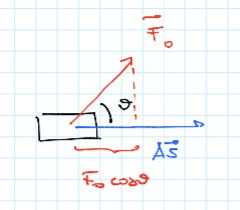
\includegraphics[width=6cm]{lezione7/images/1Precorsolavoroedenergia}\\
		\caption{Lavoro per spostare un oggetto applicando una forza costante in modulo, direzione e verso}
	\end{center}
\end{figure}
\begin{definizione}
	
	Il lavoro è dato da una forza applicata costante in modulo e direzione da 
	$$L=\vec{F}\cdot \vec{\Delta s}=F\cdot \Delta s \cdot cos \theta$$
	
Se invece la forza applicata cambia lungo una curva allora punto per punto avremo la situazione appena descritta, e passando al continuo otterremo un integrale. Nello specifico la situazione è data dalla figura 
	\begin{figure}[h!]
	\begin{center}
		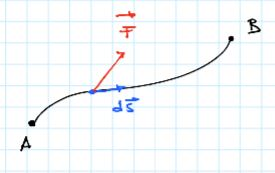
\includegraphics[width=6cm]{lezione7/images/2Precorsolavoroedenergia}\\
		\caption{Lavoro per spostare un oggetto applicando una forza costante in modulo ma non in direzione e verso, decomposizione infinitesima}
	\end{center}
\end{figure}

ed è necessario calcolare un integrale (perchè stiamo lavorando una suddivisione in tratti infinitesimi) per ottenere il lavoro lunga la curva da A a B dato da 
$$L_{AB}=\int_{A}^{B} \vec{F} \cdot d \vec{s}$$ 

Il lavoro avrà come unità di misura il Joule J, ottenuto così:
$$[L]=[F][\Delta s] = \frac{ML}{T^2} L= \frac{ML^2}{T^2} = \frac{kg \cdot m^2}{s^2}:=J$$

dove abbiamo indicato con $L$ la lunghezza, $M$ la massa e $T$ il tempo. E' importante ricordarsi che il lavoro è una quantita \textbf{scalare}.
\end{definizione}

 Possiamo analizzare i seguenti casi particolari facendo variare la direzione e verso della forza 
\begin{figure}[h]
	\begin{center}
		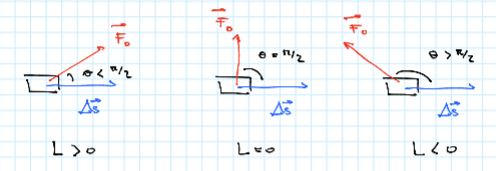
\includegraphics[width=10cm]{lezione7/images/3Precorsolavoroedenergia}\\
		\caption{Lavoro al variare dell'angolo $\theta$.}
	\end{center}
\end{figure}

Quindi parliamo di lavoro positivo, nullo e negativo rispettivamente.

\subsection{Energia cinetica}
Abbiamo introdotto il lavoro a partire dal fatto che su un oggetto spostato agisce una forza. Ma per la seconda legge di Newton, se su un corpo agisce una forza la velocità di questo oggetto varia secondo la legge $F =m\cdot a$. Allora possiamo pensare di introdurre una grandezza, in funzione della velocità, per fare in modo tale che variando la forza, anche la velocità varia di conseguenza, e quindi la grandezza definita, e cambia perché stiamo compiendo un lavoro.


\begin{esempio}
	Consideriamo un caso particolare per introdurre questa grandezza. L'esempio che consideriamo è quello del moto rettilineo uniformemente accellerato, cioè soggetto ad una forza applicata costante in modulo direzione e verso. In particolare la direzione è proprio quella del moto.
	
	\begin{figure}[h]
		\begin{center}
			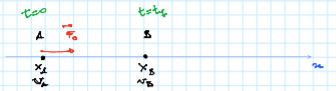
\includegraphics[width=8cm]{lezione7/images/4Precorsolavoroedenergia.jpg}\\
			\caption{Moto rettilineo uniformemente accelerato}
		\end{center}
		\end{figure}
	
	Bisogna ricordare che nel caso di moto rettilineo uniformemente accelerato valgono le relazioni
	
	$$x(t) =\frac{1}{2}at^2+v_0 t +x_0$$
	$$v(t)=at+v_0$$.
	
	Perciò se $a=F_0 /m$, $x_0 =x_A$ e $v_0 =v_A$ 
		\begin{figure}[h]
		\begin{center}
			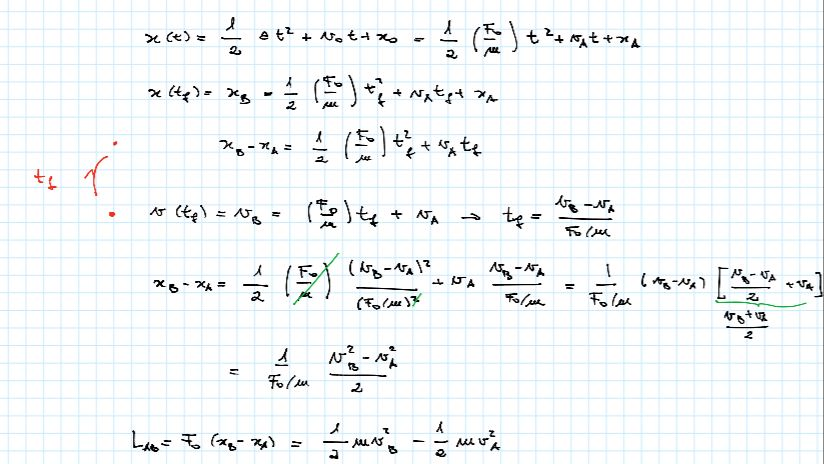
\includegraphics[width=11cm]{lezione7/images/5Precorsolavoroedenergia}\\
			\caption{Conti}
		\end{center}
	\end{figure}
\end{esempio}

\begin{definizione}
	L'energia cinetica viene definita come 
	$$E_k=\frac{1}{2}mv^2$$
	
	La sua unità di misura è ancora il Joule e si ha che 
	
	$$L_{AB}=E_k (B)- E_k (A)$$ 
	e quest'ultima è una relazione generale.
\end{definizione}

\subsection{Forze conservative ed energia potenziale}

\begin{definizione}
Una forza si dice conservativa se il lavoro svolto non dipende da una particolare curva ma solamente dai punti iniziali e finali. 
\end{definizione}
	\begin{figure}[h]
	\begin{center}
		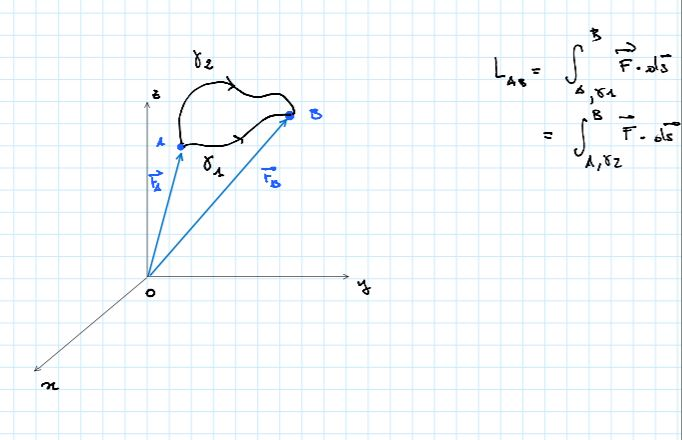
\includegraphics[width=8cm]{lezione7/images/6Precorsolavoroedenergia}\\
		\caption{Cammini chiusi.}
	\end{center}
\end{figure}

\begin{esempio}[La forza peso è conservativa]
	\begin{figure}[h]
	\begin{center}
		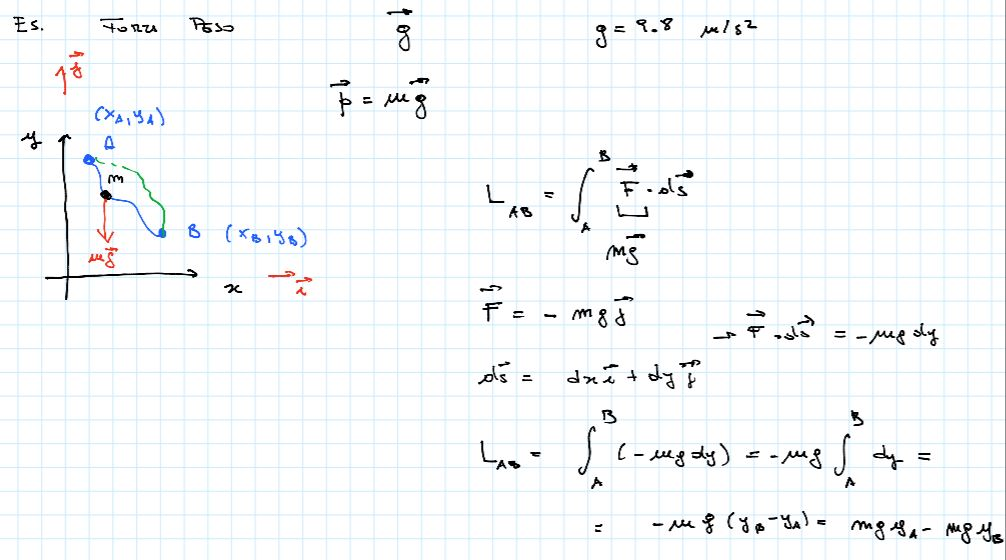
\includegraphics[width=10cm]{lezione7/images/7Precorsolavoroedenergia}\\
		\caption{Lavoro della forza peso}
	\end{center}
\end{figure}

\end{esempio}

Se una forza è conservativa, perciò dipende solo dalla posizione iniziale e finale e possiamo introdurre una funzione della sola coordinata spaziale, la posizione, detta \textit{Energia potenziale}. Cioè stiamo dicendo che nel caso di una forza conservativa 
$$L_{AB}=\int_{A}^{B} \vec{F}\cdot d \vec{s} = E_p (A)- E_p (B)$$

Dove con il simbolo $E_p$ indichiamo l'energia potenziale in un certo punto (quindi funzione solo della posizione). 

\begin{itemize}
\item Questa funzione è definita solo a meno di una costante additiva, in quanto definita tramite una differenza, quindi la costante non influisce in alcun modo. Infatti se sostituisco $E_p (\vec{r})$ con $E_p (\vec{r})+E_{p,0} $ allora $E' _p (A)=E_p (A)+E_{p,0} $, $E' _p (B)=E_p (B)+E_{p,0} $ e resta definita la differenza in quanto 
$$E' _p (A) - E' _p (B)= E' _p (A)=E_p (A)+E_{p,0} -(E_p (B)+E_{p,0}) = E _p (A) - E _p (B)$$

\item Abbiamo espresso il lavoro come variazione di energia potenziale dal punto iniziale al punto finale e non viceversa, perciò stiamo 'scegliendo' un segno. Lo facciamo in questo modo perché il lavoro che una forza $F$ compie per spostare  un oggetto da A a B, è uguale ed opposto a quello di una agente esterno che vuole portarlo da B ad A. Allora questa inversione inverte gli estremi dell'integrale che definisce il lavoro, allora inverte un segno. Allora se la forza è conservativa il lavoro che l'esterno fa contro la forza $F$ per uno spostamento da B ad A se è positivo l'energia potenziale dell'oggetto spostato è aumentata (che è quello che penseremo intuitivamente).
\item Nel caso di forze conservative il lavoro su spostamenti nulli è ovviamente nullo. Cioè se punto iniziale e finale sono uguali, il lavoro è nullo.
\end{itemize}

Quindi in generale abbiamo che il lavoro può essere espresso tramite 
$$L_{AB}=E_k (B)- E_k (A)$$ 

Nel caso particolare di forze conservative abbiamo 
$$L_{AB}= E_p (B)- E_p (A)$$

che deve dunque essere uguale alla prima espressione richiamata

$$E_k (B)- E_k (A)= E_p (B)- E_p (A)$$ 

da cui 


\begin{proposizione}[Conservazione dell'energia]
	L'energia totale/meccanica per forze conservative si conserva, cioè vale che 
	
	$$E_k (B)+E_p (B)= E_k (A)+E_p (A)$$ 
\end{proposizione}

\begin{esempio}
	Un carrello scivola avanti e indietro lungo un binario liscio posto in un piano verticale. la forma del binario è parabolica e la quota in funzione della positione orizzontale è $y=kx^2$ con $k=0,92$.
	\begin{enumerate}
		\item Trovare le coordinate $x$ dei punti di inversione del moto se la velocità massima del carrello vale $v_{max}=8,5 m/s$.
		\item Trovare il modulo della velocità del carrello quando si trova a metà dell'altezza massima.
	\end{enumerate}
	\begin{figure}[h]
	\begin{center}
		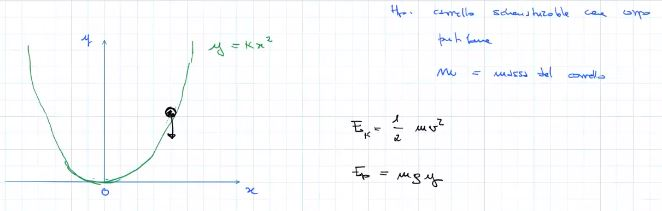
\includegraphics[width=12cm]{lezione7/images/8Precorsolavoroedenergia.jpg}\\
		\caption{Rappresentazione del problema.}
	\end{center}
\end{figure}
	\begin{figure}[h]
	\begin{center}
		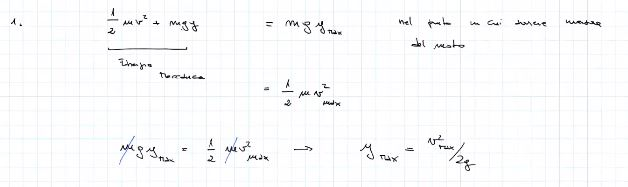
\includegraphics[width=12cm]{lezione7/images/9Precorsolavoroedenergia.jpg}\\
		\caption{}
	\end{center}
\end{figure}

	\begin{figure}[h]
	\begin{center}
		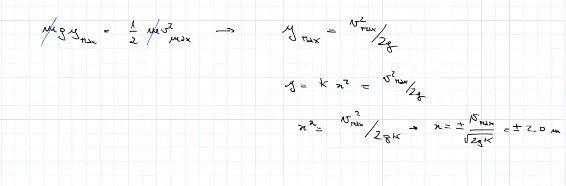
\includegraphics[width=12cm]{lezione7/images/10Precorsolavoroedenergia.jpg}\\
		\caption{Svolgimento punto 1.}
	\end{center}
\end{figure}

	\begin{figure}[h]
	\begin{center}
		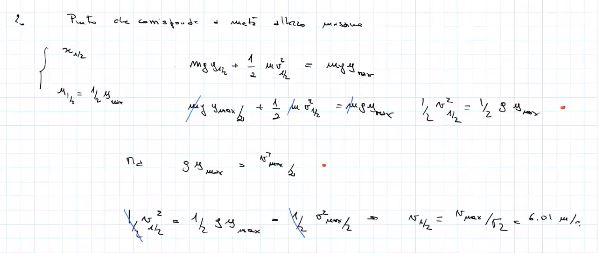
\includegraphics[width=12cm]{lezione7/images/11Precorsolavoroedenergia.jpg}\\
		\caption{Svolgimento punto 2}
	\end{center}
\end{figure}

\end{esempio}
